\documentclass[final]{beamer}

\usepackage[scale=1.24]{beamerposter}
\usetheme{confposter}
\setbeamercolor{block title}{fg=ngreen,bg=white}
\setbeamercolor{block body}{fg=black,bg=white}
\setbeamercolor{block alerted title}{fg=white,bg=dblue!70}
\setbeamercolor{block alerted body}{fg=black,bg=dblue!10}

\newlength{\sepwid}
\newlength{\onecolwid}
\newlength{\twocolwid}
\newlength{\threecolwid}
\setlength{\paperwidth}{48in} % A0 width: 46.8in
\setlength{\paperheight}{34in} % A0 height: 33.1in
\setlength{\sepwid}{0.024\paperwidth} % Separation width (white space) between columns
\setlength{\onecolwid}{0.22\paperwidth} % Width of one column
\setlength{\twocolwid}{0.464\paperwidth} % Width of two columns
\setlength{\threecolwid}{0.708\paperwidth} % Width of three columns
\setlength{\topmargin}{-0.5in} % Reduce the top margin size
%-----------------------------------------------------------

\usepackage{graphicx}  % Required for including images

\usepackage{booktabs} % Top and bottom rules for tables

\usepackage{hyperref}
\hypersetup{
    colorlinks=true,
    linkcolor=blue,
    filecolor=magenta,      
    urlcolor=blue,
}

\usepackage{amsmath}

\title{Close Encounter: 456938 (2007 YV56) } % Poster title

\author{Bosscha Observatory $\vert$ Astronomy Research Division, ITB}

\institute{This information is generated on 2017-09-07 17:28 UTC.} 

\begin{document}

\addtobeamertemplate{block end}{}{\vspace*{2ex}}
\addtobeamertemplate{block alerted end}{}{\vspace*{2ex}}

\setlength{\belowcaptionskip}{2ex}
\setlength\belowdisplayshortskip{2ex}

\begin{frame}[t]

\begin{columns}[t] 

% First Column

\begin{column}{\sepwid}\end{column}

\begin{column}{\onecolwid}

\begin{alertblock}{Basic Properties}
\begin{itemize}
\item Name: 456938 (2007 YV56)\item Discovered 2007-Dec-31 by CSS at Catalina 
\item Estimated diameter: 167 \--- 375 meters
\item Classification: Apollo (NEO, PHA)
\item H: 21.0
\item Period: 722.345 days
\end{itemize}
\begin{table}
\caption{Orbital elements at epoch 2458000.5 JD }
\begin{tabular}{l c r}
\toprule
\textbf{Parameter} & & \textbf{    Value    } \\
\midrule Semi-major axis ($a$) & & 1.57554 \\ 
Eccentricity ($e$) & & .622205 \\ 
Inclination ($i$) & & 6.24408 \\ 
Lon. of ascending node ($\Omega$) & & 102.423 \\ 
Argument of pericenter ($\omega$) & & 265.730 \\ 
Mean Anomaly ($M$) & & 348.294 \\ 
\bottomrule
\end{tabular}
\end{table}

\end{alertblock}


\begin{block}{Orbit}
\begin{figure}
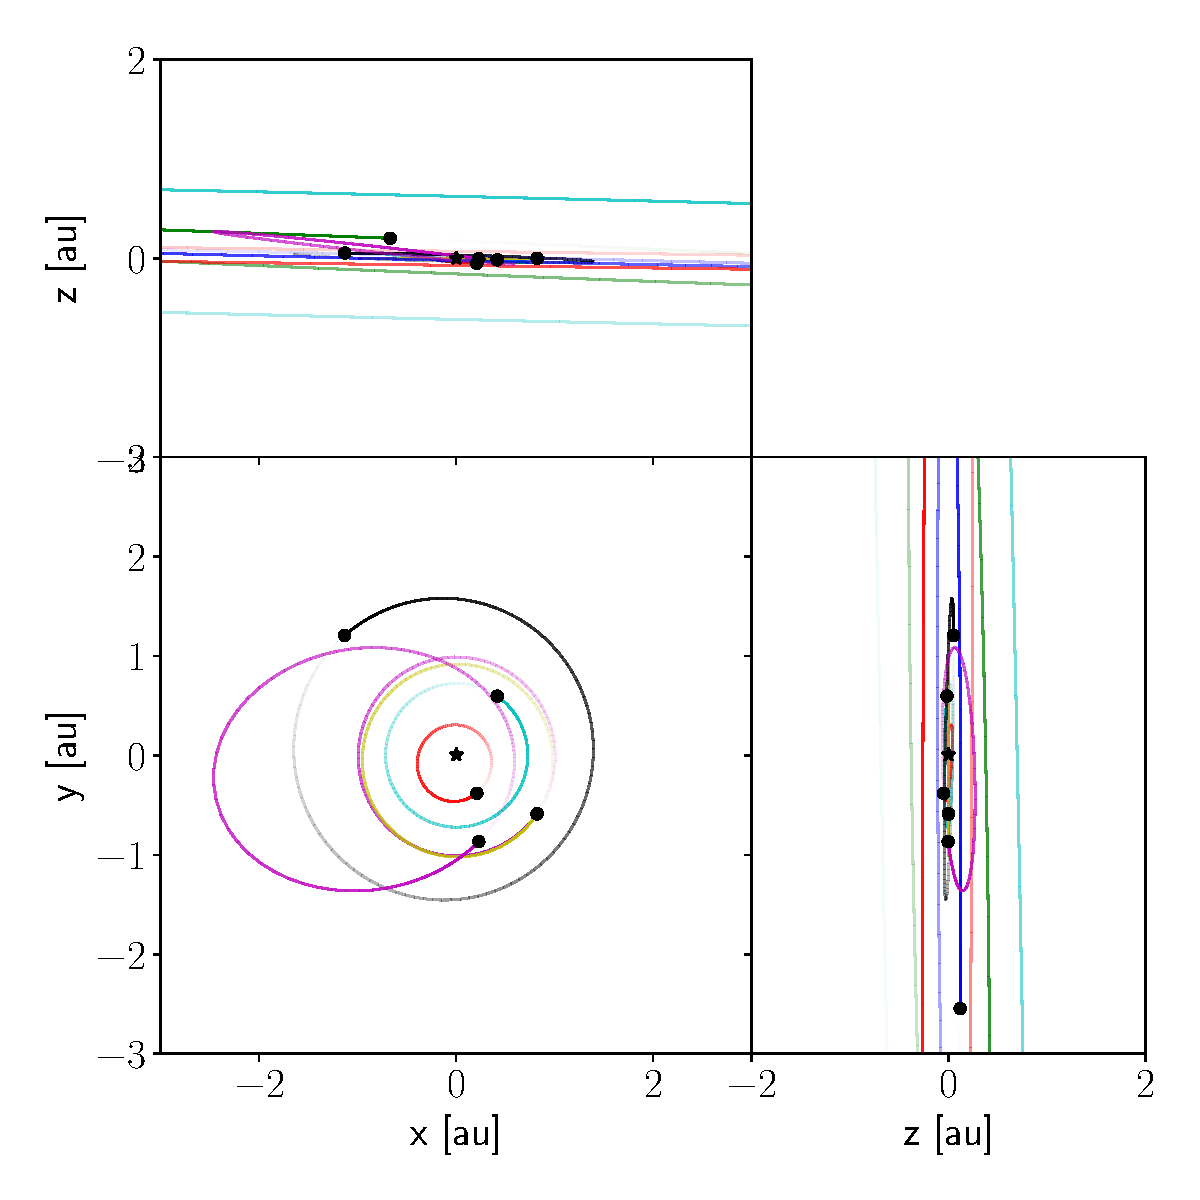
\includegraphics[width=0.99\textwidth]{initial_orbit.pdf}
\caption{Orbit of the asteroid and the planets. This plot only shows the inner region of the Solar System.}
\end{figure}
\end{block}

\begin{alertblock}{Acknowledgements}
Our script retrieve basic informations and initial condition from \href{https://ssd.jpl.nasa.gov/}{JPL NASA}, re-integrate the Solar System using \href{https://github.com/hannorein/rebound}{\texttt{Rebound}} package, and write this report using \LaTeX.
\end{alertblock}

\end{column}

% Second column

\begin{column}{\sepwid}\end{column}

\begin{column}{\twocolwid}

\begin{block}{Distance to the Earth and Orbital Elements}
\begin{figure}
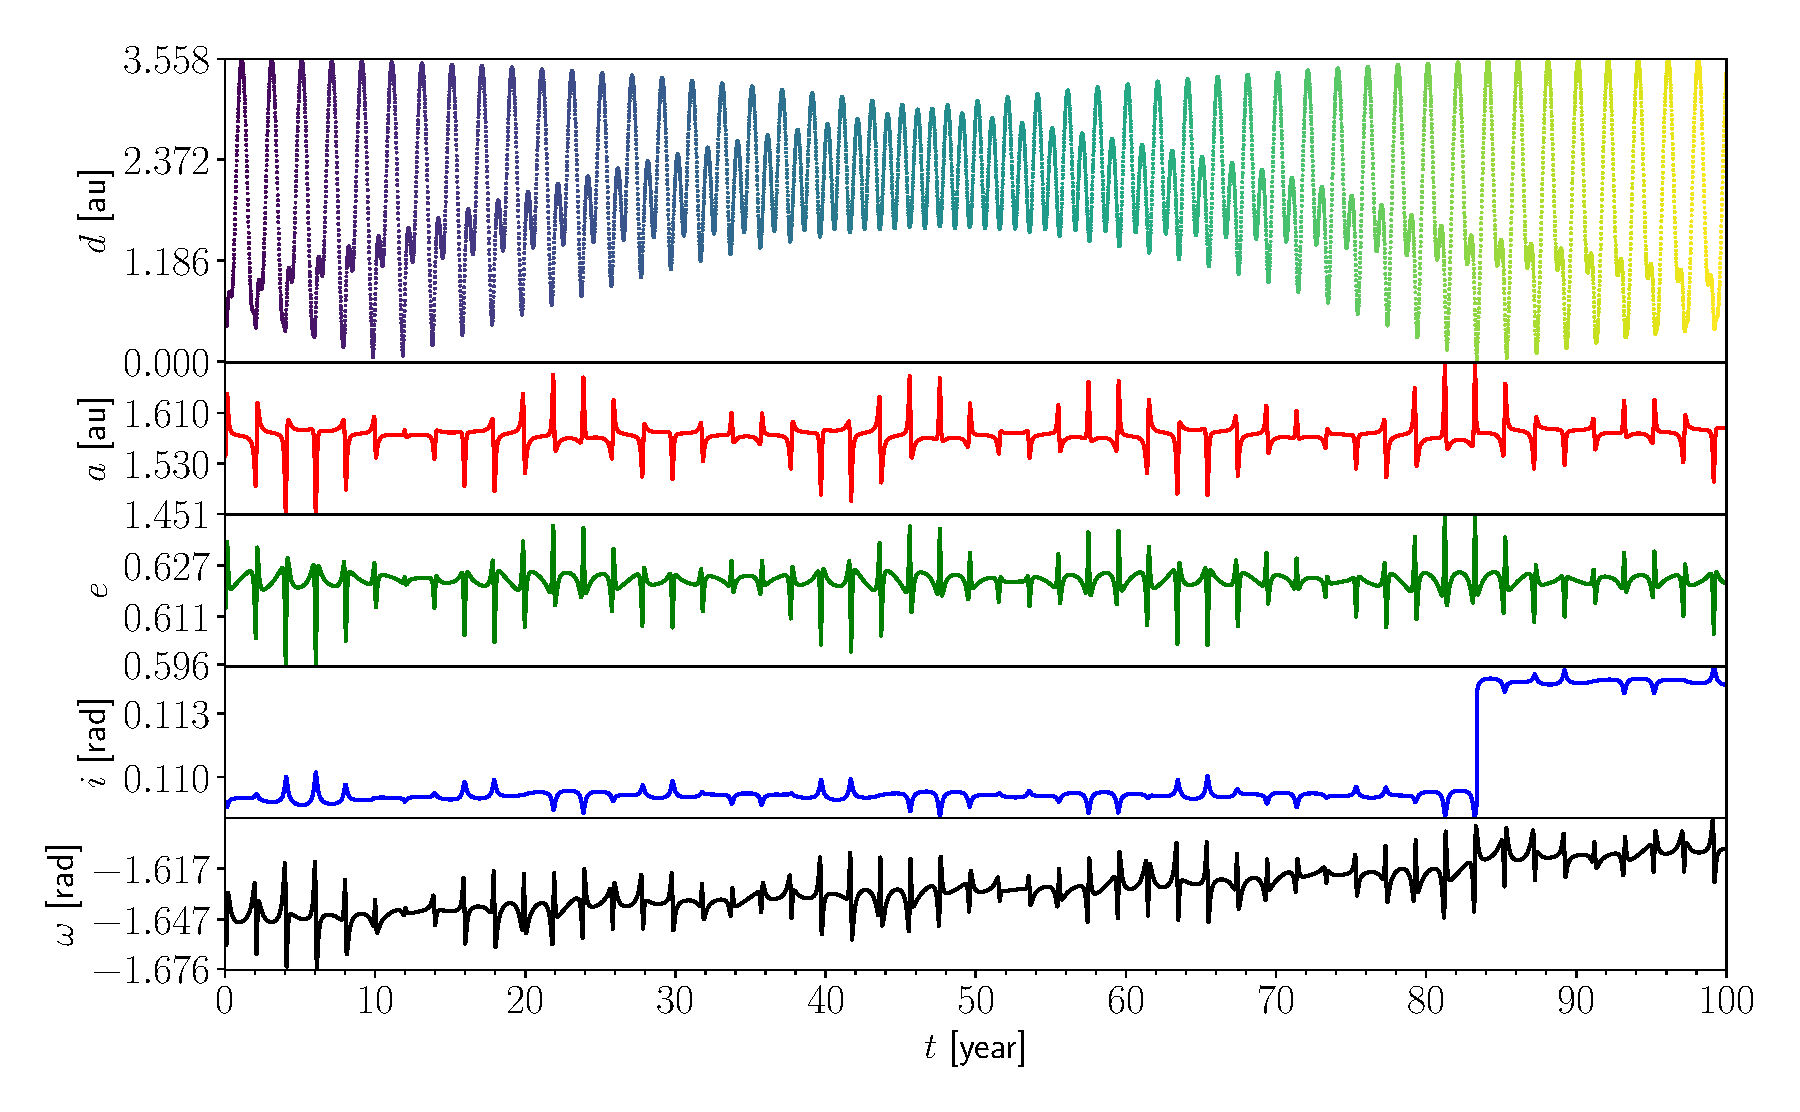
\includegraphics[width=0.99\linewidth]{daeiw.pdf}
\caption{Distance to the Earth and orbital elements of the asteroid for the next 100 years. Starting time of the integration is 2017-08-17 00:00 UTC.}
\end{figure}
\end{block}

\begin{columns}[t, totalwidth=\twocolwid] % Split up the two columns wide column

\begin{column}{\onecolwid}\vspace{-.6in}
\begin{block}{Geocentric}
\begin{figure}
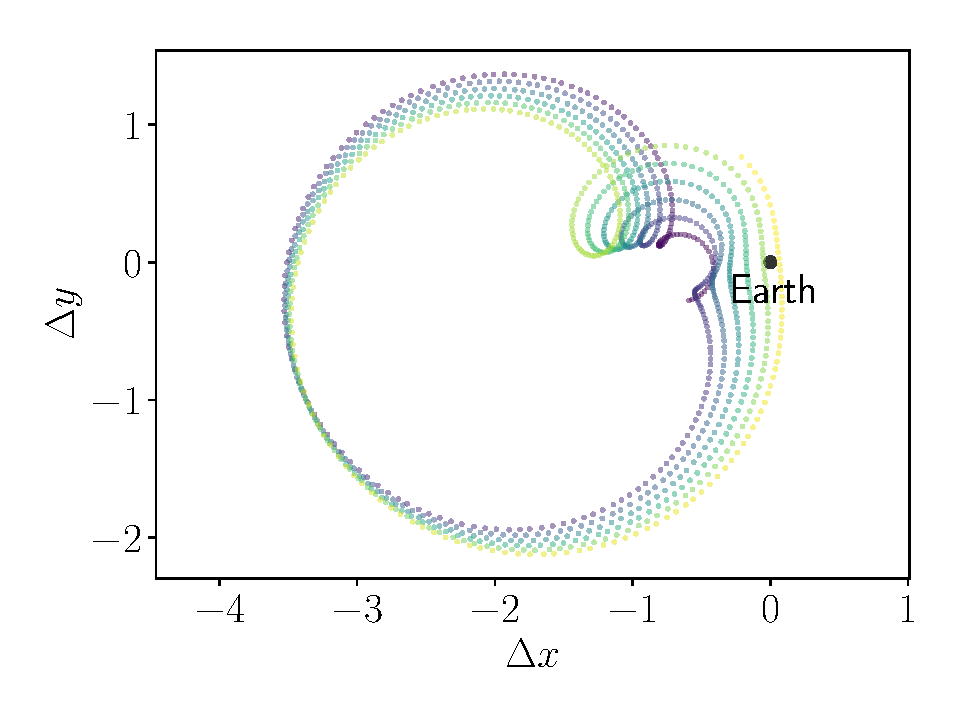
\includegraphics[width=0.99\textwidth]{geocentric.pdf}
\caption{Movement of the asteroid relative to the Earth ($xy$-plane; only the first 12 years of integration).}
\end{figure}
\end{block}
\end{column}

\begin{column}{\onecolwid}\vspace{-.6in} 
\begin{block}{Rotating Frame}
\begin{figure}
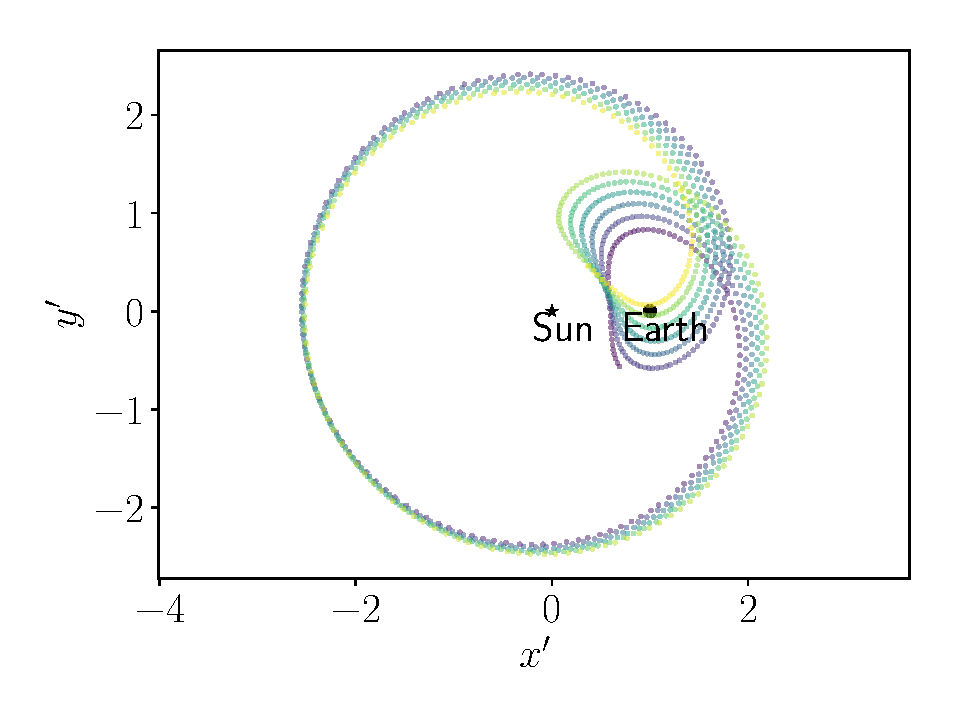
\includegraphics[width=0.99\textwidth]{rotframe.pdf}
\caption{Movement of the asteroid relative to the Sun-Earth system ($xy$-plane; only the first 12 years of integration).}
\end{figure}
\end{block}
\end{column}

\end{columns} 

\end{column} 


%%%% 
\begin{column}{\sepwid}\end{column} 

\begin{column}{\onecolwid} 

\setbeamercolor{block alerted title}{fg=black,bg=norange}
\setbeamercolor{block alerted body}{fg=black,bg=norange!10}

\begin{alertblock}{Nearest close encounter}
\begin{itemize}
\item Time: 1 September 2017, 12.05 UT
\item Distance:  $ 7.066 \times 10^6$ km ($18.38$ Lunar Distance)
\item Relative velocity: 
\end{itemize}
\end{alertblock}


\begin{alertblock}{List of close encounter}
\begin{table}
\vspace{2ex}
\begin{tabular}{l c c c}
\toprule
\textbf{Time} & \textbf{   Body   } & \textbf{  $\boldsymbol{d}$ (au)  } & \textbf{$\boldsymbol{v_{rel}}$ (km/s)} \\
\midrule2017-09-24 & Earth & 0.4142 & 19.34 \\ 
2019-09-08 & Earth & 0.3987 & 18.23 \\ 
2021-08-20 & Earth & 0.3611 & 15.93 \\ 
2023-07-29 & Earth & 0.2888 & 12.91 \\ 
2023-08-13 & Venus & 0.0596 & 14.47 \\ 
2025-07-07 & Earth & 0.1735 & 14.20 \\ 
2027-06-28 & Earth & 0.0503 & 17.78 \\ 
2029-06-22 & Earth & 0.0660 & 20.99 \\ 
2031-06-16 & Earth & 0.1904 & 24.66 \\ 
2033-06-09 & Earth & 0.3140 & 28.31 \\ 
2033-08-21 & Venus & 0.0389 & 16.86 \\ 
2035-06-04 & Earth & 0.4327 & 31.90 \\ 
2041-06-02 & Venus & 0.0901 & 21.45 \\ 
2047-10-03 & Mars & 0.0675 & 13.71 \\ 
2051-05-26 & Venus & 0.1328 & 14.19 \\ 
2069-02-23 & Venus & 0.0773 & 13.91 \\ 
2079-03-03 & Venus & 0.0470 & 18.32 \\ 
2085-05-16 & Mars & 0.0705 & 13.66 \\ 
2086-12-16 & Venus & 0.0258 & 18.34 \\ 
2095-01-22 & Earth & 0.4226 & 31.99 \\ 
2096-12-04 & Venus & 0.1314 & 14.12 \\ 
2097-01-14 & Earth & 0.2828 & 27.69 \\ 
2099-01-08 & Earth & 0.1371 & 23.27 \\ 
2101-01-02 & Moon & 0.0019 & 18.80 \\ 
2101-01-02 & Earth & 0.0015 & 19.27 \\ 
2102-12-31 & Earth & 0.0435 & 17.85 \\ 
2104-10-13 & Venus & 0.1398 & 23.76 \\ 
2104-12-27 & Earth & 0.1006 & 16.18 \\ 
2106-12-23 & Earth & 0.1630 & 14.34 \\ 
2108-12-14 & Earth & 0.2271 & 12.72 \\ 
2110-11-30 & Earth & 0.2876 & 12.97 \\ 
2114-11-15 & Venus & 0.1482 & 23.90 \\ 
2130-08-24 & Venus & 0.0100 & 16.71 \\ 
2134-08-24 & Earth & 0.3635 & 16.03 \\ 
2136-08-20 & Earth & 0.3524 & 15.43 \\ 
2138-08-15 & Venus & 0.1227 & 22.92 \\ 
2138-08-15 & Earth & 0.3371 & 14.68 \\ 
2140-08-09 & Earth & 0.3194 & 13.87 \\ 
2154-12-22 & Mars & 0.0787 & 14.79 \\ 
2164-07-04 & Earth & 0.1030 & 16.20 \\ 
2166-07-05 & Earth & 0.1076 & 16.05 \\ 
2168-07-05 & Earth & 0.1128 & 15.90 \\ 
2170-07-06 & Earth & 0.1263 & 15.55 \\ 
2172-07-07 & Earth & 0.1437 & 15.04 \\ 
2174-07-09 & Earth & 0.1607 & 14.54 \\ 
2176-07-11 & Earth & 0.1831 & 13.94 \\ 
2178-07-14 & Earth & 0.2078 & 13.31 \\ 
\bottomrule
\end{tabular}
%\caption{Word Formation}
\end{table}
\end{alertblock}

\end{column} 


\end{columns} 
\end{frame}
\end{document}